RHODES approach to traffic signal optimization is a hierachical one with 3 layers of detail, see figure \ref{fig:rhodes_hierarchi}. They can be rougly be summarized accordingly:

\begin{enumerate}
\item The macroscopic layer performs \textit{dynamic network loading}, which involves observing changes in the aggregated flow data of the entire network and updating of OD matrices. This layer supplies estimates of link flows to the middle level in rough numbers eg. vehicles per hour.
\item The mesoscopic middle layer considers sectors of the network eg. an arterial. This \textit{network flow control} layer work in the detail level of platoons and average speeds. Green time is allocated to phases to accomodate the movements of the platoons and so coordination of signals is done at this level.
\item At the lowest level is \textit{intersection control} where vehicles are handled individually (a microscopic layer). Here the green times and phase ordering suggested by the middle layer are fine tuned.
\end{enumerate}

\begin{figure}[!ht]
\begin{center}
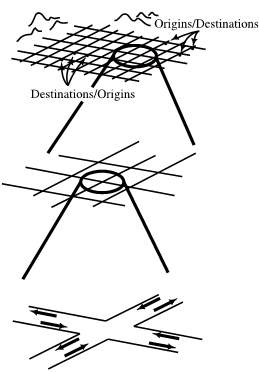
\includegraphics[scale=0.5]{rhodes_hierachy.png} 
\end{center}
\caption{The three levels of detail: network, sector, and intersection}
\label{fig:rhodes_hierarchi}
\end{figure}

RHODES must operate quickly in order to adapt signals to traffic in real-time. This platform has good decomposition opportunities and is pluggable ie. the upper level is a black box feeding the lower level with predictions and optimizations.

\subsubsection*{Detection}


\subsubsection*{Prediction}

\subsubsection*{Optimization}

\subsubsection*{Evaluation}
